%%%%%%%%%%%%%%%%%%%%%%%%%%%%%%%%%%%%%%%%%%%%%%%%%%%%%%%%
%%%%%%                                            %%%%%%
%%%                                                  %%%
%      Modèle de Rapport.                              %
%               Par Matthieu Maury                     %
%                                                      %
%%%                                                  %%%
%%%%%%                                            %%%%%%
%%%%%%%%%%%%%%%%%%%%%%%%%%%%%%%%%%%%%%%%%%%%%%%%%%%%%%%%

\documentclass[10pt, a4paper]{report}

%%%%%%%%%%%%%%%%%%%%%%%%%%%%%%%%%%%%%%%%%%%%%%%%%%%%%%%%
%% Package essentiel
\usepackage[greek,english]{babel}
\usepackage[T1]{fontenc}
\usepackage{ucs}
\usepackage[utf8x]{inputenc}
\usepackage[top=2.6cm,bottom=2.6cm,right=2.1cm,left=2.1cm]{geometry}
\usepackage{float}

%%%%%%%%%%%%%%%%%%%%%%%%%%%%%%%%%%%%%%%%%%%%%%%%%%%%%%%%
%% Package optionnel
\usepackage{enumerate}
\usepackage{graphicx}
\usepackage{tabularx}
\usepackage{setspace}
\usepackage[dvips]{pstricks}
\usepackage{pstricks-add}
\usepackage{color}
\usepackage{xcolor}
\usepackage{epsfig}
\usepackage{pst-grad} % For gradients
\usepackage{pst-plot} % For axes
\usepackage{amsmath}
\usepackage{amsfonts}
\usepackage{amssymb}
\usepackage{amsxtra}
\usepackage{mathrsfs}
\usepackage{framed}
%\usepackage[framed, thmmarks, amsmath]{ntheorem}
\usepackage{verbatim}
\usepackage{moreverb}
\usepackage{fancyhdr}
\usepackage{url}
\usepackage{listings}
%\usepackage{hyperlinks}
\usepackage{lettrine}

%%%%%%%%%%%%%%%%%%%%%%%%%%%%%%%%%%%%%%%%%%%%%%%%%%%%%%%%
%%%%%%                                            %%%%%%
%%         Configuration de la mise en page           %%
%%%%%                                              %%%%%
%%%%%%%%%%%%%%%%%%%%%%%%%%%%%%%%%%%%%%%%%%%%%%%%%%%%%%%%

%%%%%%%%%%%%%%%%%%%%%%%%%%%%%%%%%%%%%%%%%%%%%%%%%%%%%%%%
%% Profondeur du sommaire
\setcounter{secnumdepth}{4}
\setcounter{tocdepth}{4}

%%%%%%%%%%%%%%%%%%%%%%%%%%%%%%%%%%%%%%%%%%%%%%%%%%%%%%%%
%% Configuration des chapitres
\makeatletter
\def\@makechapterhead#1{%
  \vspace*{50\p@}%
  {\parindent \z@ \raggedright \normalfont
    \interlinepenalty\@M
    \Huge \bfseries\thechapter.\quad#1\par\nobreak
    \vskip 20\p@
  }}
\makeatother

%%%%%%%%%%%%%%%%%%%%%%%%%%%%%%%%%%%%%%%%%%%%%%%%%%%%%%%%
%%%%%%                                            %%%%%%
%%                Début du Document                   %%
%%%%%                                              %%%%%
%%%%%%%%%%%%%%%%%%%%%%%%%%%%%%%%%%%%%%%%%%%%%%%%%%%%%%%%


\lstset{tabsize=3, inputencoding=utf8x, extendedchars=\true, language=C}

%% Symboles des ensembles
\newcommand{\R}{\ensuremath{\mathbb{R}} }
\newcommand{\N}{\ensuremath{\mathbb{N}} }
\newcommand{\Z}{\ensuremath{\mathbb{Z}} }
\newcommand{\Q}{\ensuremath{\mathbb{Q}} }
\newcommand{\C}{\ensuremath{\mathbb{C}} }
\newcommand{\U}{\ensuremath{\mathbb{U}} }
\newcommand{\K}{\ensuremath{\mathbb{K}} }

%% Symboles mathématique
\newcommand{\spi}{\ensuremath{\Pi} } %Pi
\newcommand{\sqqs}{\ensuremath{\forall} } %quelque soit
\newcommand{\sex}{\ensuremath{\exists} } %il existe
\newcommand{\snex}{\ensuremath{\nexists} }
\newcommand{\simpld}{\ensuremath{\Rightarrow} } %implique vers la droite
\newcommand{\simplg}{\ensuremath{\Leftarrow} } %implque vers la gauche
\newcommand{\sequ}{\ensuremath{\Leftrightarrow} }
\newcommand{\sand}{\ensuremath{\wedge} }
\newcommand{\sou}{\ensuremath{\vee} }
\newcommand{\smneg}{\ensuremath{\neg} }
\newcommand{\snimpld}{\ensuremath{\nRightarrow} } %implique vers la droite
\newcommand{\snimplg}{\ensuremath{\nLeftarrow} } %implque vers la gauche
\newcommand{\snequ}{\ensuremath{\nLeftrightarrow} }
\newcommand{\sinclut}{\ensuremath{\in} }
\newcommand{\sninclut}{\ensuremath{\notin} }
\newcommand{\sposd}{\ensuremath{\owns} }
\newcommand{\ssups}{\ensuremath{\supset} }
\newcommand{\snsups}{\ensuremath{\nsupset} }
\newcommand{\ssubs}{\ensuremath{\subset} }
\newcommand{\ssubeq}{\ensuremath{\subseteq} }
\newcommand{\ssupeq}{\ensuremath{\supseteq} }
\newcommand{\snsubeq}{\ensuremath{\nsubseteq} }
\newcommand{\snsupeq}{\ensuremath{\nsupseteq} }
\newcommand{\sneg}{\ensuremath{\neq} }
\newcommand{\saprox}{\ensuremath{\approx} }
\newcommand{\ssim}{\ensuremath{\sim} }
\newcommand{\scompl}[2]{\ensuremath{\complement_{#1}{#2}} }
\newcommand{\sunion}{\ensuremath{\cup} }
\newcommand{\sinters}{\ensuremath{\cap} }
\newcommand{\sx}{\ensuremath{\times} }
\newcommand{\svide}{\ensuremath{\emptyset} }
\newcommand{\Pa}{\ensuremath{\mathcal{P}} }
\newcommand{\lra}{\ensuremath{\longrightarrow}}
\newcommand{\rond}{\ensuremath{\circ} }
\newcommand{\frestric}[2]{\ensuremath{#1|_{#2}} }
\newcommand{\sbar}[1]{\ensuremath{\overline{#1}}}
\newcommand{\si}{\ensuremath{\imath}}
\newcommand{\zl}[1]{\ensuremath{\mathscr{#1}}}
\newcommand{\stimes}{\ensuremath{\times}}
\newcommand{\classe}[1]{\ensuremath{\overset{\bullet}{#1}}}


\begin{document}

%%%%%%%%%%%%%%%%%%%%%%%%%%%%%%%%%%%%%%%%%%%%%%%%%%%%%%%%
%% Inclusion de la page de titre
\pagestyle{fancy}
\renewcommand{\sectionmark}[1]{\markright{\thesection\ #1}}
\renewcommand{\footrulewidth}{0pt}
\renewcommand{\headrulewidth}{0pt}
\fancyhead{} % clear all header fields
\fancyfoot{} % clear all footer fields
\fancyfoot[LO,RE]{\textit{University year 2009-2010}}
\fancyfoot[LE,RO]{\textit{Written with \LaTeX}}

\begin{tabularx}{17cm}{Xr}
  \begin{tabular}{ll}
    Yohann Teston & 881003-P792\\
    \url{yohann.teston@free.fr} &\\
	Matthieu Maury & 860928-P210\\
	\url{mayeu.tik@gmail.com} & \\
  \end{tabular} 

  &
  
  \begin{tabular}{r}
    
\includegraphics[width=5cm]{pic/logoupp.eps} \\
    \textit{Department of Information Technology} \\
  \end{tabular}
\end{tabularx}

\vspace{6cm}

\begin{center}
  \textbf{ {\Huge Programming of parallel computers}}\\[0.5em]{\huge Assignment 1 - MPI}
\end{center}

\begin{center}
  \today
\end{center}


\newpage


\thispagestyle{empty}
%\input{resume}

\renewcommand{\footrulewidth}{0.5pt}
\renewcommand{\headrulewidth}{0.5pt}
\fancyhead{} % clear all header fields
\fancyhead[RE,LO]{Secure Computer Systems - Assignment 1}


\fancyhead[RO,LE]{\rightmark}

\fancyfoot{} % clear all footer fields
\fancyfoot[LO,RE]{Group 9: Manohar Kaul \& Murat Ayfer \& Yohann Teston}
\fancyfoot[LE,RO]{\thepage}

%Redéfinition du style fancy - plain, utilisé pour les pages de nouveau chapitre
%Le style par défaut est un style plain
\fancypagestyle{plain}{
    \fancyhf{}
    \renewcommand{\headrulewidth}{0pt}

    %Définition des headers identiques à une page normale
    \fancyfoot[LO,RE]{Group 9: Manohar Kaul \& Murat Ayfer \& Yohann Teston}
    \fancyfoot[LE,RO]{\thepage}
}

\tableofcontents

%\listoffigures

%\newpage

%\doublespacing
\onehalfspacing
\chapter{Compile and run MPI programs}

As expected, running the unmodified hello program results in several \textit{Hello World!} being printer, one for each processor we are running on.

After modification of the program, we have the following result:
\begin{figure}[!h]
\begin{center}
	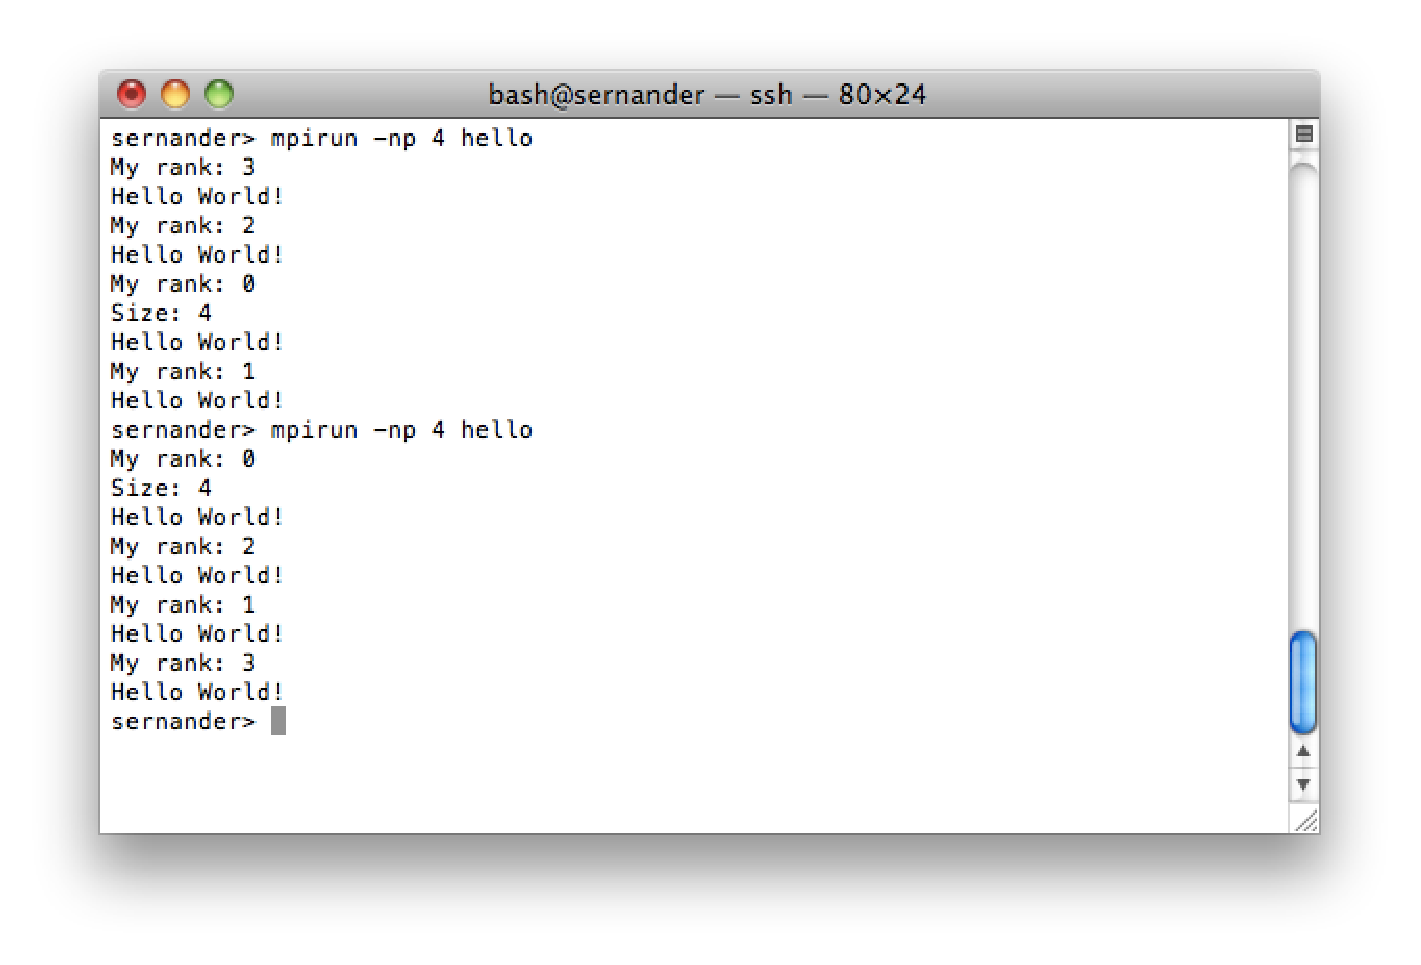
\includegraphics[width=\textwidth]{pic/hello.eps}
	\caption{Result of the modified hello program}
\end{center}
\end{figure}

We can see that only the processor with rank 0 prints the number of processors. The picture also shows that there is no pre-defined order between the processors because the order of the messages changes. This is normal because the processes created are scheduled independly on their processor. So, there is no way to tell which one will start first or in which order the result will appear.


\chapter{Point-to-point communication}

\section{Work on \textit{exchange.c}}

The main advantage of using non-blocking calls is that it becomes possible to overlap communication and computation. Indeed, those calls start the process of sending or receiving and return without completing it. The caller is then free to do some other computation during the communication and is not blocked until the end of the communication, as it is the case with a blocking call. The main drawback is that the programmer must make sure not to alter the sending/receiving buffer because they are being used even after the non-blocking call has returned. This makes programming harder.

\section{Work on \textit{pingpong.c}}

By tracing the data we obtain:

%\begin{figure}[h]
  \begin{center}
	 \psfig{figure=pic/ex2.eps}
  \end{center}
%  \caption{}
%  \label{fig:}
%\end{figure}

The average latency is: $6.8794us$. And the average bandwidth: $522.1591 MB.s^{-1}$.

The graph is linear, showing that the latency between sending and receiving a message is constant during the whole send/reicv programm.


\chapter{Collective communication, global data}

\section{Pass-on}

As can be seen in the following picture, the \textit{pass-on} method has been successfully implemented. For a better understanding of what is going on, the messages have been labelled with the rank of the sender. Thus, we can see that the value is correctly passed from a processor to its direct neighbor.
\begin{figure}[!h]
\begin{center}
	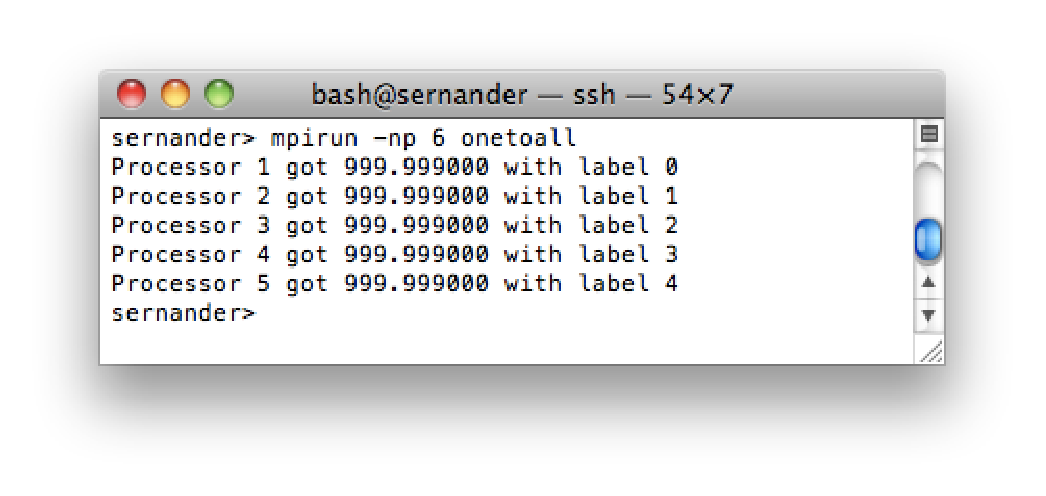
\includegraphics[width=\textwidth]{pic/passon.eps}
	\caption{Pass-on}
\end{center}
\end{figure}

\section{Fan-out}

\begin{verbatim}
Lain-ux@nyarlathothep:code > mpirun -np 8 a.out 
Processor 1 got 999.999000 from 0
Processor 2 got 999.999000 from 0
Processor 3 got 999.999000 from 1
Processor 4 got 999.999000 from 0
Processor 5 got 999.999000 from 1
Processor 6 got 999.999000 from 2
Processor 7 got 999.999000 from 3
\end{verbatim}

\section{Broadcast}

The following picture allows us to verify the correctness of the program using \textit{MPI\_Bcast}.
\begin{figure}[!h]
\begin{center}
	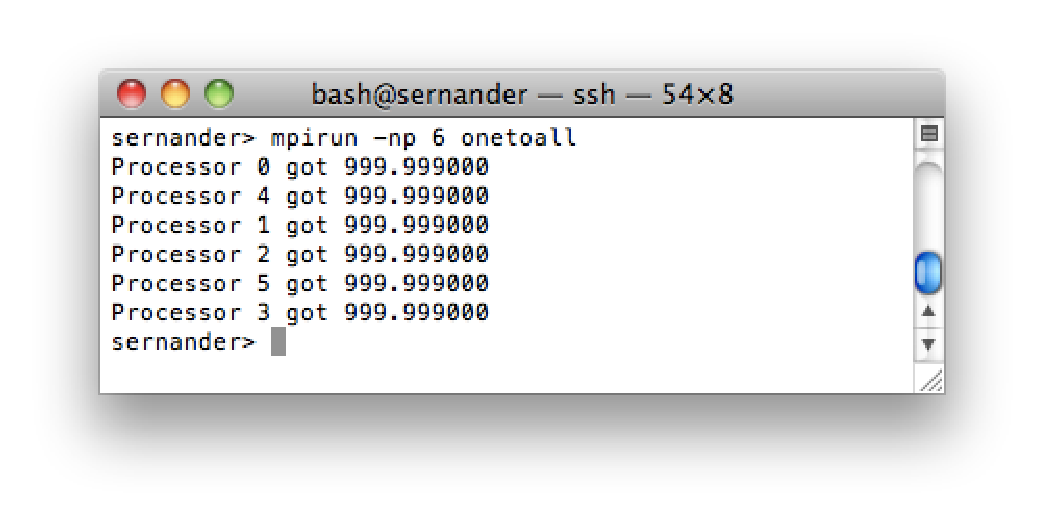
\includegraphics[width=\textwidth]{pic/bcast.eps}
	\caption{Broadcast}
\end{center}
\end{figure}

MPI does have a lot of other \textit{collective communication} operations, described as follows:

\begin{itemize}
	\item Barrier synchronization across all group members
	\item Broadcast from one member to all members of a group
	\item Gather data from all group members to one member 
	\item Scatter data from one member to all members of a group
	\item A variation on Gather where all members of the group receive the result
	\item Scatter/Gather data from all members to all members of a group
	\item Global reduction operations such as sum, max, min, or user-defined functions, where the result is returned to all group members and a variation where the result is returned to only one member (used in the following exercise) 
	\item A combined reduction and scatter operation
	\item Scan across all members of a group (also called prefix)
\end{itemize}

\chapter{Reduction, global operations}

In this exercise, we used the MPI function \textit{MPI\_Reduce} with the reduce operation \textit{MPI\_SUM}. The result of the program is shown by the following picture:
\begin{figure}[!h]
\begin{center}
	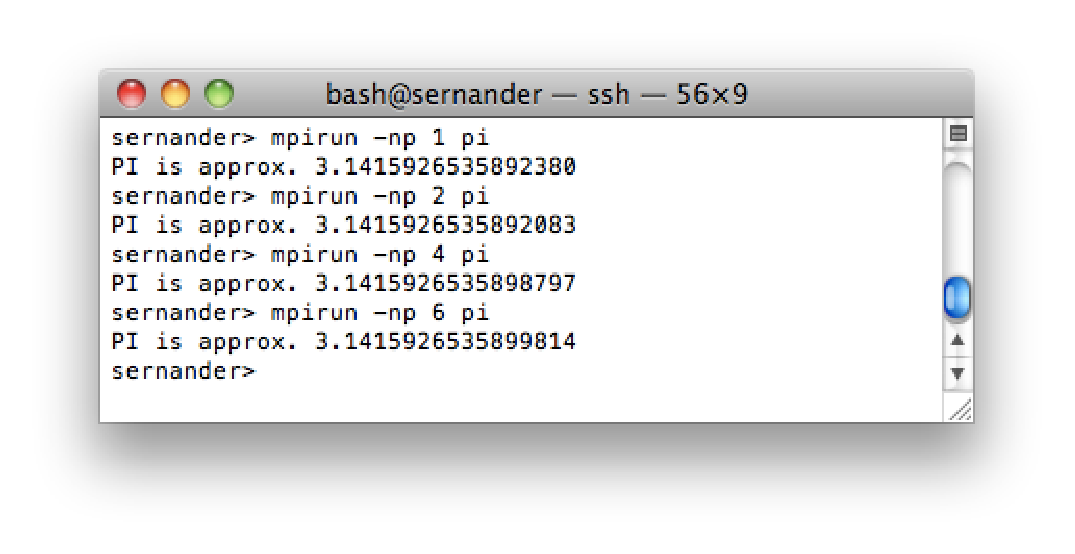
\includegraphics[width=\textwidth]{pic/pi.eps}
	\caption{Value of $\pi$ on a different number of processors}
\end{center}
\end{figure}

The results are a correct approximation of $\pi$, proof that the program does what it is designed for.


\chapter{Derived datatypes}

The function \textit{MPI\_Type\_vector} allows the user to create a derived datatype. In our case, we want to create a datatype representing the quater of a matrix having \textit{nx} lines and \textit{ny} columns.

The main parameters are defined as follows (given a type for the elements in the array, like \textit{MPI\_Double} in our case):
\begin{description}
	\item[count:] indicates the number of blocks in our datatype
	\item[blocklength:] indicates the length of a block
	\item[stride:] indicates the number of elements between the beginning of each block
\end{description}
So, when we will ask the system to transer such a datatype, it will transfer \textit{count} blocks of \textit{blocklength} elements, the first element of each block being separated from the next one by \textit{stride} elements. Thus, using the values \textit{count} = \textit{nx}/2, \textit{blocklength} = \textit{ny}/2 and \textit{stride} = \textit{ny}, we get a derived datatype representing a quater of our matrix.

The result of the program being huge, it has not been included here.


\chapter{Communicators}

In the unmodified program, the process on the row being at the rank 0, that is in the column 0 since column number are used for ordering, transfers the row number to the other process in the same row. So, all the processes on a row will have their row number as data, as can be seen in the followig picture:
\begin{figure}[!h]
\begin{center}
	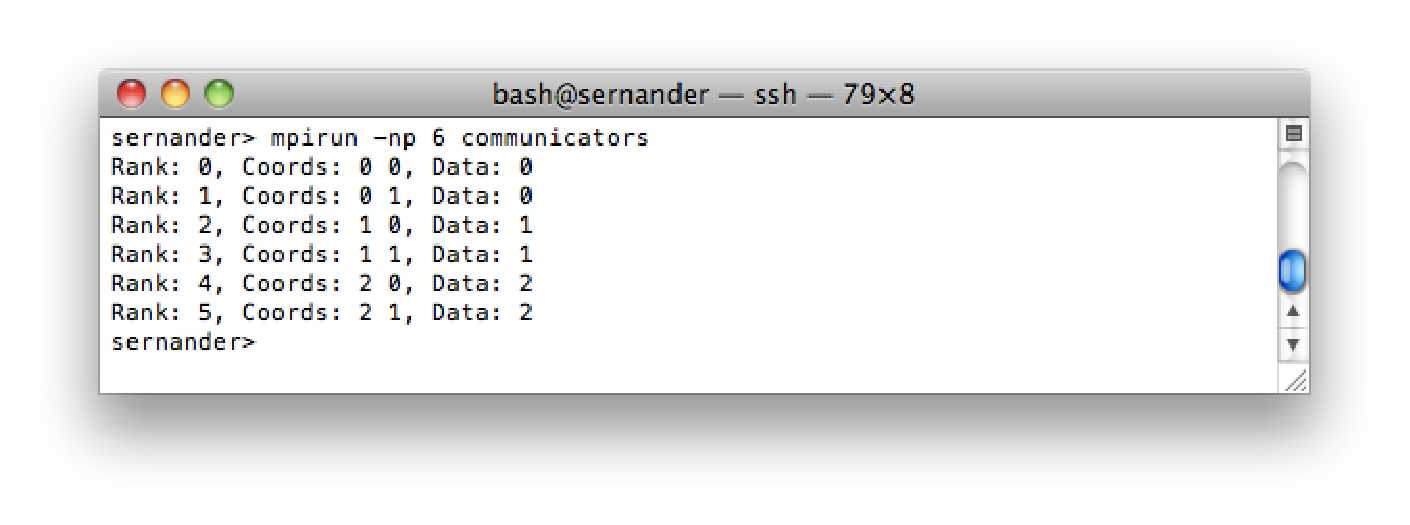
\includegraphics[width=\textwidth]{pic/row.eps}
	\caption{Communicator for each row}
\end{center}
\end{figure}

In the modified program, the communicator is declared in such a way that processes are grouped by column number and sorted by row number (the exact opposite as before). So, now, the first process of a column, the one being on the row 0, sends its row number to the processes in the same column. So, the value of every process becomes the row number of the rank 0 process in this column, that is 0. This is illustrated by the following screenshot:
\begin{figure}[!h]
\begin{center}
	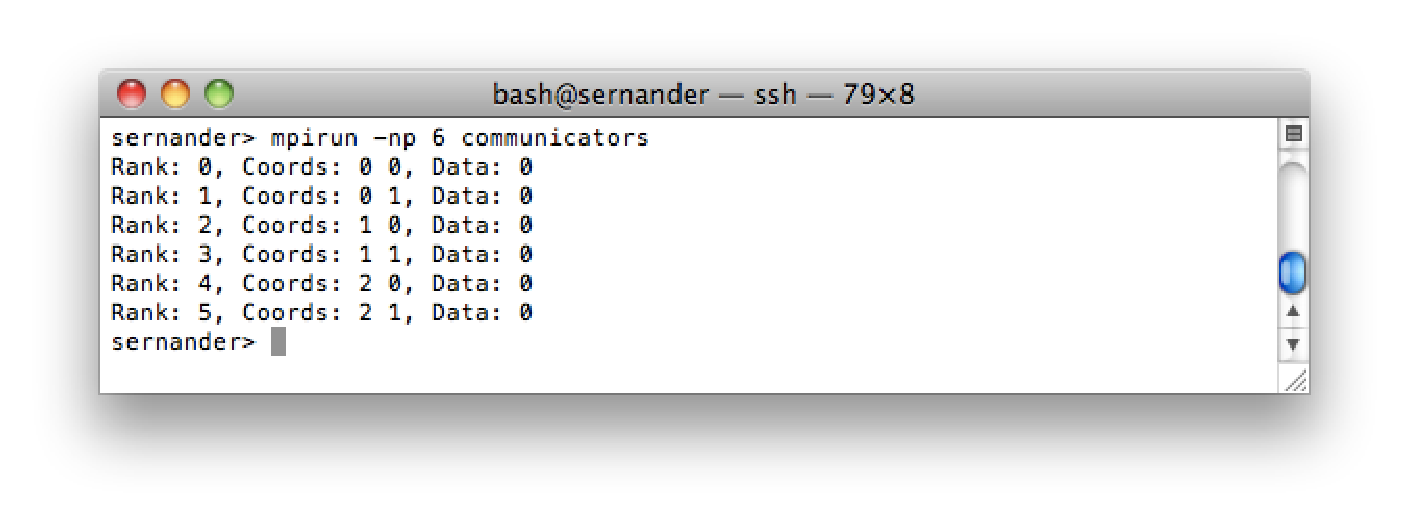
\includegraphics[width=\textwidth]{pic/col.eps}
	\caption{Communicator for each column}
\end{center}
\end{figure}


\chapter{PDE solver}

The program has been run twenty times using a different number of processors each time. The results are listed in the table below:

\begin{center}
\begin{tabular}{|c|c|}
\hline
Numbers of processors & Time to complete \\
\hline
1 & 51.8073 \\
2 & 28.1724 \\
4 & 15.9394 \\
6 & 11.5323 \\
8 & 9.6533 \\
10 & 7.35941 \\
15 & 5.14445 \\
16 & 4.5774 \\
20 & 4.25137 \\ 
24 & 3.20059 \\ 
28 & 3.30171 \\
30 & 3.08664 \\
32 & 2.75156 \\
35 & 2.47561 \\
40 & 2.24806 \\
42 & 2.20288 \\
48 & 1.90164 \\
53 & 1.58522 \\
59 & 1.46382 \\
64 & 1.52331 \\
\hline
\end{tabular}
\end{center}

Using those data, it is possible to compute the \textit{speedup}. The picture \ref{graph} shows it.

\begin{figure}[!h]
\begin{center}
	\includegraphics[width=\textwidth]{pic/graph.ps}
	\caption{Speedup graph}
	\label{graph}
\end{center}
\end{figure}

When we double the number of processors allocated to the program, we could expect that it will only need half of the time it needed previously. As we can see on the graphic, this is not true. Indeed, using 64 processors is only about 34 times faster than using one processor where we could have expected a program 64 times faster. 

The problem is the more processors we use the more communications we do. Those communications introduce a lot of overheads. So, a part of the time won by having a new processor working on the program is spent setting the communications and doing some others things that must be done but does not produce a useful result. This is why the speedup is not what we could have expected.
 


%\newpage
%\setcounter{page}{1}
%\pagenumbering{Roman}
%\appendix
%\chapter{Source code}

\lstinputlisting{../fox.c}

\chapter{Time result}

\section{Result}
\verbatiminput{pic/result.dat}

\section{GNUplot script}
\lstset{language=Gnuplot}
\lstinputlisting{pic/graph.gpi}

\chapter{Launching script}

\lstset{language=Ruby}
\lstinputlisting{../launch.rb}


\end{document}
